\documentclass[14pt]{beamer}

\title[A Tour of Go]{\huge Let's Go!}
\author{Mansi Sharma}
\usetheme{Madrid}

\definecolor{deepblue}{HTML}{302B70}

\begin{document}

{
\begin{frame}
    \titlepage
    
\includegraphics[width=\linewidth]{img/golang.png}
\end{frame}
}

{
\begin{frame}
    \frametitle {What is Go?}
    \begin{center}
        \textcolor{deepblue}{Go is a \textcolor{red}{compiled}, \textcolor{green}{concurrent}, \textcolor{yellow}{garbage-collected}, \textcolor{blue}{statically typed} language developed at}
        \linebreak
        
\includegraphics[width=0.3\linewidth]{img/google.png}
    \end{center}
\end{frame}
}

{
\begin{frame}
    \frametitle{Features of Go}
    \begin{columns}
        \begin{column}{0.5\textwidth}
            \begin{itemize}
                \item Open-source Project
                \item Compiled language
                \item Easy concurrency support via goroutines
                \item Package Management
                \item Static typing
            \end{itemize}
        \end{column}
        \begin{column}{0.5\textwidth}
            \begin{itemize}
                \item Features powerful standard library
                \item Garbage collection called goLand
                \item Great libraries
                \item Easy and readable code
            \end{itemize}
        \end{column}
    \end{columns}
\end{frame}
}

{
\begin{frame}
    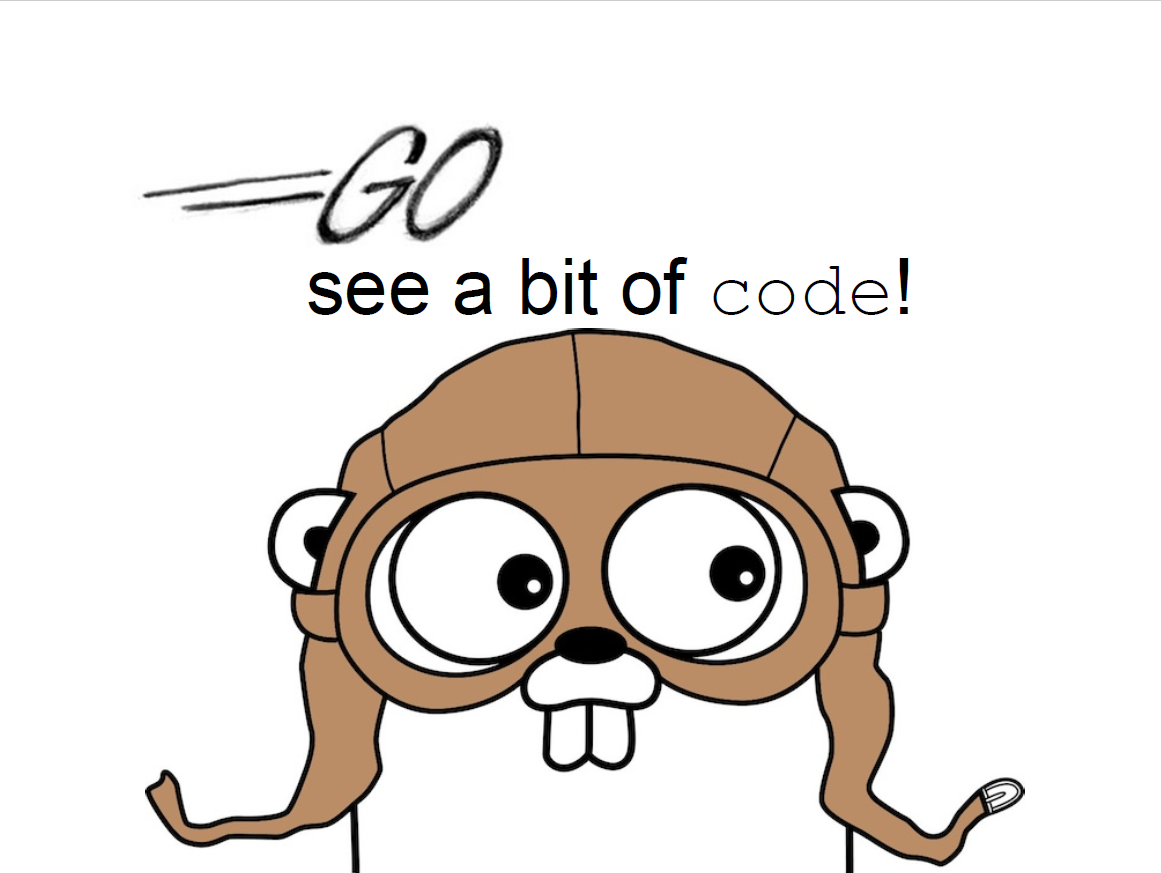
\includegraphics[width=\linewidth]{img/golang.PNG}
\end{frame}
}

{
\begin{frame}
    \frametitle{Hello, World!}
    \begin{itemize}
        \item Programs start running in package main.
        \item It is good style to use the factored import statement.
        \item A name is exported if it begins with a capital letter.
    \end{itemize}
    \begin{center}
        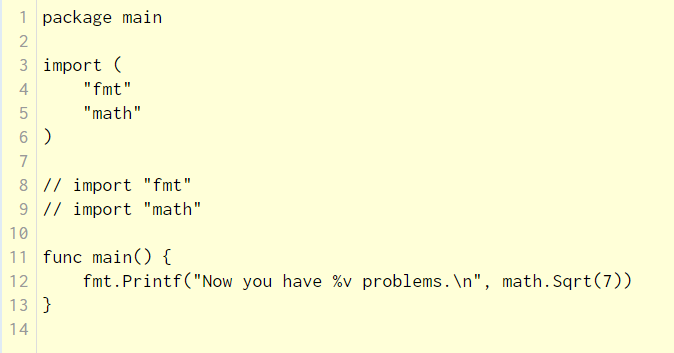
\includegraphics[width=0.7\linewidth]{img/introtogo.PNG}
    \end{center}
\end{frame}
}

{
\begin{frame}
    \frametitle{Variables}
    \begin{itemize}
        \item The var instruction declares a list of variables
        \item The type is informed at the end
        \item The var instruction could includes initializers, 1 per variable. In this case, the type could be ommited
    \end{itemize}
    \begin{center}
        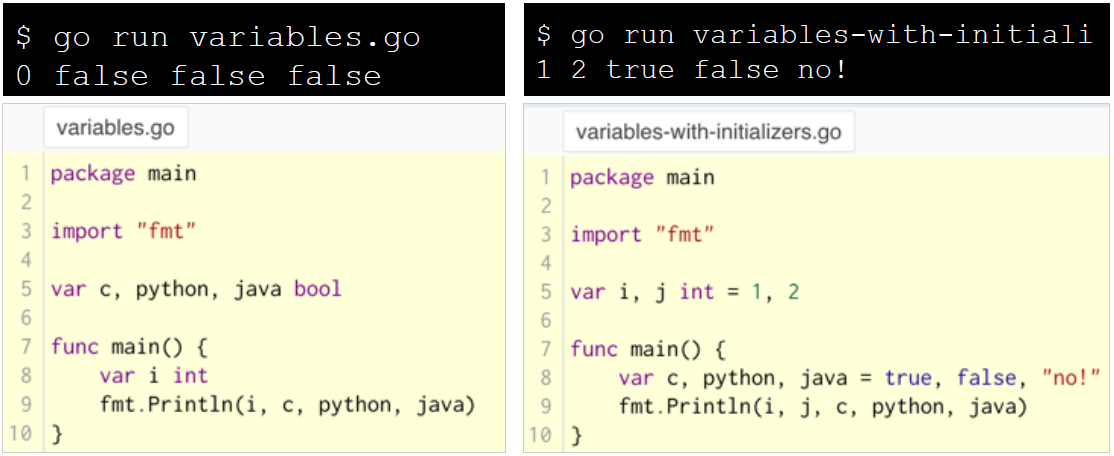
\includegraphics[width=\linewidth]{img/variables.PNG}
    \end{center}
\end{frame}
}

{
\begin{frame}
    \frametitle{Short Variable Declarations}
    \begin{itemize}
        \item Inside a function, the short attribution instruction := can be used instead of a var declaration
    \end{itemize}
    \begin{center}
        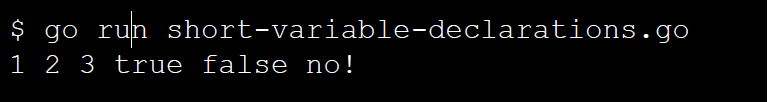
\includegraphics[width=0.6\linewidth]{img/shortdeclarationcommand.PNG}
        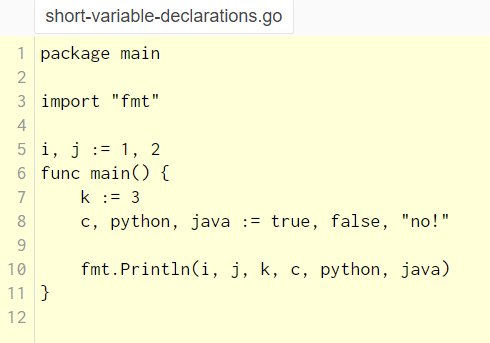
\includegraphics[width=0.6\linewidth]{img/shortdeclaration.PNG}
    \end{center}
\end{frame}
}

{
\begin{frame}
    \frametitle{Constants}
    \begin{itemize}
        \item Constants are declared like variables but with keyword const
        \item Can not use the syntx :=
    \end{itemize}
    \begin{center}
        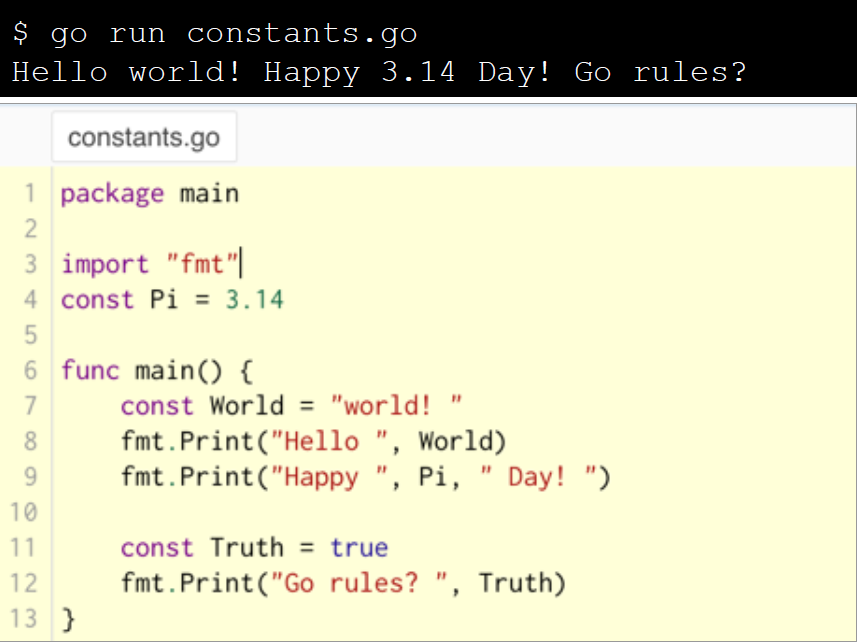
\includegraphics[width=0.6\linewidth]{img/constants.PNG}
    \end{center}
\end{frame}
}

{
\begin{frame}
    \frametitle{Functions}
    \begin{itemize}
        \item Type comes after the parameter name, like variables
        \item Shorten (x int, y int) to (x, y int)
    \end{itemize}
    \begin{columns}
        \begin{column}{0.5\textwidth}
            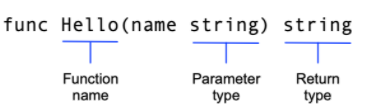
\includegraphics[width=\linewidth]{img/function.PNG}
            \linebreak
            \linebreak
            \linebreak
            \linebreak
            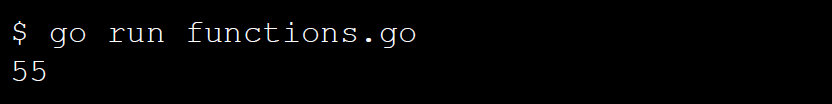
\includegraphics[width=\linewidth]{img/functionscommand.PNG}
        \end{column}
        \begin{column}{0.5\textwidth}
            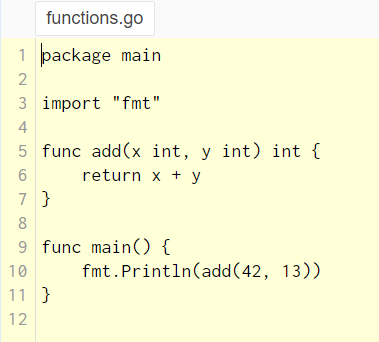
\includegraphics[width=\linewidth]{img/functions.PNG}
        \end{column}
    \end{columns}
\end{frame}
}

{
\begin{frame}
    \frametitle{Multiple Return Values}
    \begin{itemize}
        \item A function can have multiple return values
    \end{itemize}
    \begin{center}
        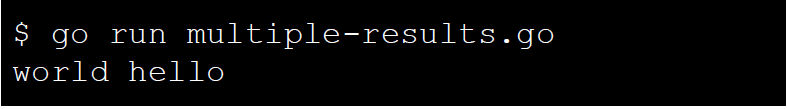
\includegraphics[width=0.65\linewidth]{img/multipleresultscommand.PNG}
        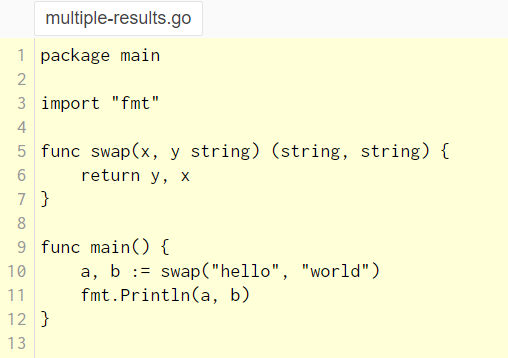
\includegraphics[width=0.65\linewidth]{img/multipleresults.PNG}
    \end{center}
\end{frame}
}

{
\begin{frame}
    \frametitle{Looping For}
    \begin{itemize}
        \item Go has only one looping construct, the for loop
        \item No parentheses required, braces are always required
        \item The init and post statements are optional
    \end{itemize}
    \begin{center}
        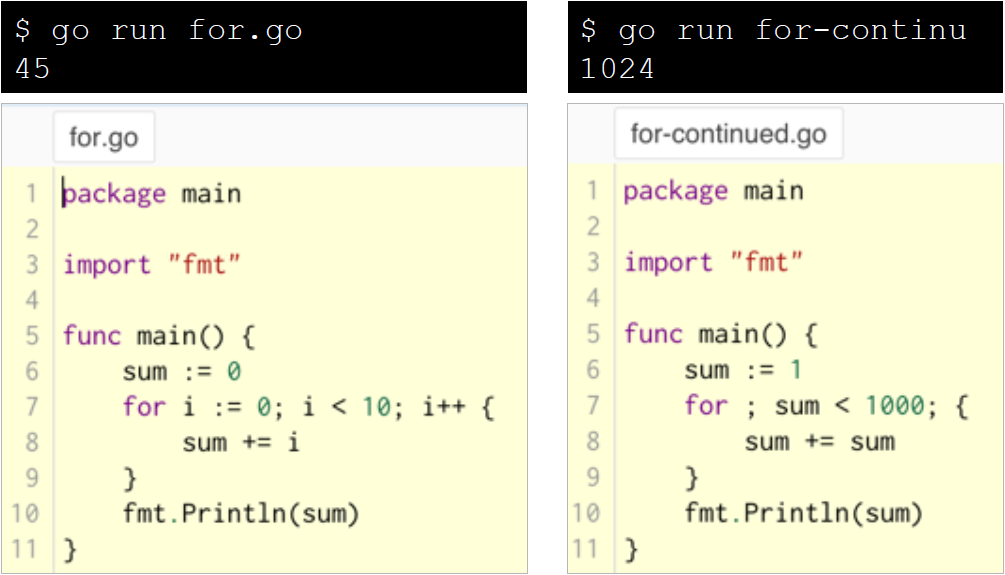
\includegraphics[width=0.8\linewidth]{img/for.PNG}
    \end{center}
\end{frame}
}

{
\begin{frame}
    \frametitle{For is Go's "while" and forever}
    \begin{itemize}
        \item Semicolon can be removed and you will have while
        \item for can run forever
    \end{itemize}
    \begin{center}
        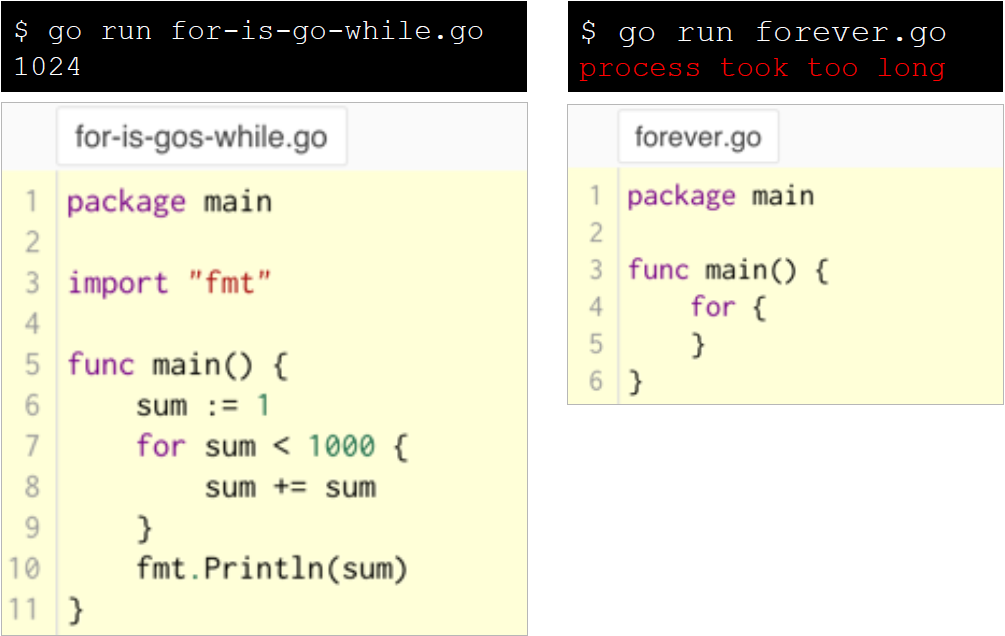
\includegraphics[width=0.8\linewidth]{img/while.PNG}
    \end{center}
\end{frame}
}

{
\begin{frame}
    \frametitle{if Condition}
    \begin{itemize}
        \item No parentheses required, braces are always required
    \end{itemize}
    \begin{columns}
        \begin{column}{0.5\textwidth}
            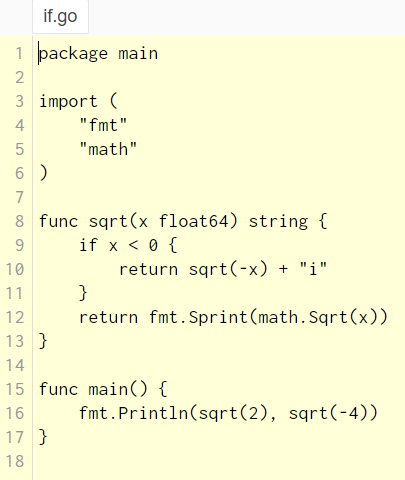
\includegraphics[width=\linewidth]{img/if.PNG}
        \end{column}
        \begin{column}{0.5\textwidth}
            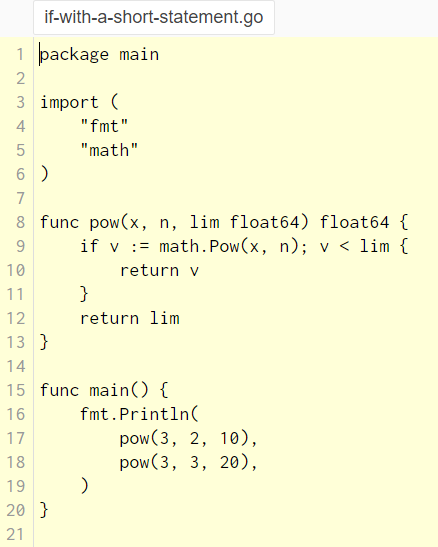
\includegraphics[width=0.9\linewidth]{img/ifshort.PNG}
        \end{column}
    \end{columns}
\end{frame}
}

{
\begin{frame}
    \frametitle{Switch}
    \begin{itemize}
        \item only runs the selected case, not all the cases that follow
        \item break statement is not required
    \end{itemize}
    \begin{columns}
        \begin{column}{0.5\textwidth}
            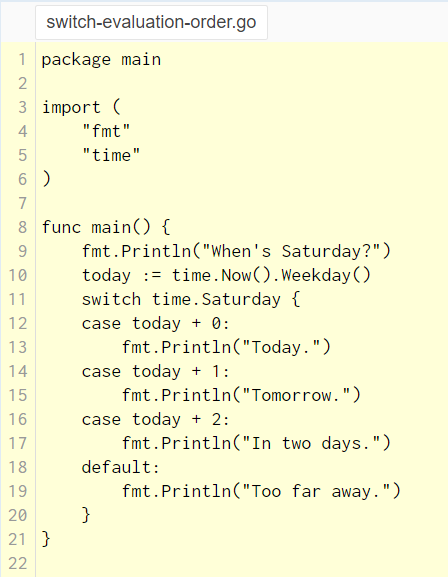
\includegraphics[width=0.75\linewidth]{img/switch1.PNG}
        \end{column}
        \begin{column}{0.5\textwidth}
            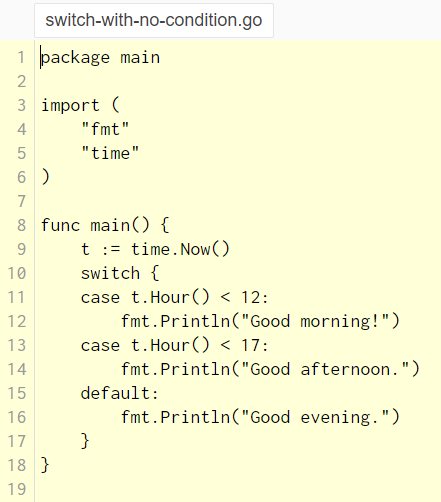
\includegraphics[width=0.8\linewidth]{img/switch2.PNG}
        \end{column}
    \end{columns}
\end{frame}
}

{
\begin{frame}
    \frametitle{Defer}
    \begin{itemize}
        \item Semicolon can be removed and you will have while
        \item for can run forever
    \end{itemize}
    \begin{center}
        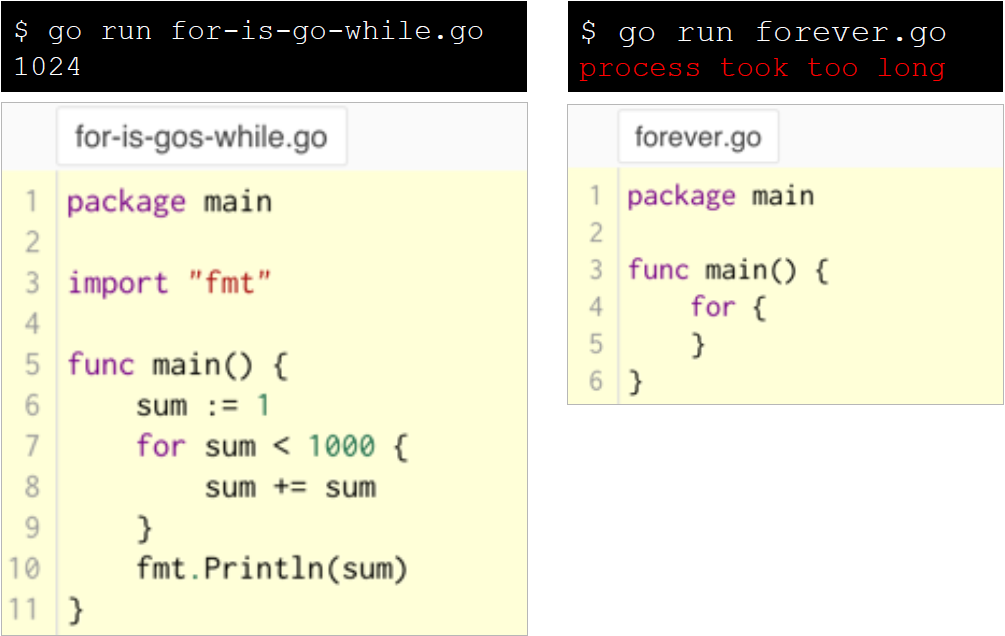
\includegraphics[width=0.8\linewidth]{img/while.PNG}
    \end{center}
\end{frame}
}

{
\begin{frame}
    \frametitle{Stacking Defer}
    \begin{itemize}
        \item Deferred function calls are pushed onto a stack
    \end{itemize}
    \begin{columns}
        \begin{column}{0.5\textwidth}
            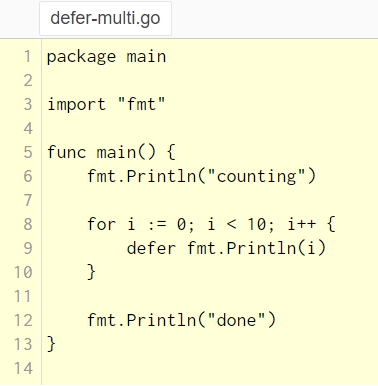
\includegraphics[width=0.9\linewidth]{img/stackdefer.PNG}
        \end{column}
        \begin{column}{0.5\textwidth}
            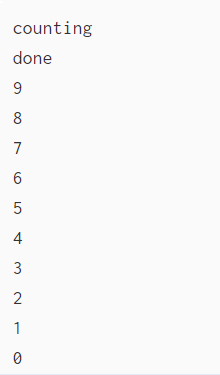
\includegraphics[width=0.5\linewidth]{img/defeeoutput.PNG}
        \end{column}
    \end{columns}
\end{frame}
}

{
\begin{frame}
    \frametitle{Pointers}
    \begin{itemize}
        \item Syntax for pointers is the same as in C or C++
        \item But unlike C, Go has no pointer arithmetic.
    \end{itemize}
    \begin{center}
        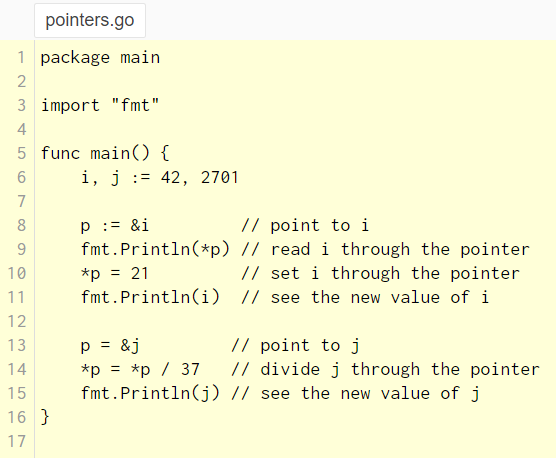
\includegraphics[width=0.6\linewidth]{img/pointers.PNG}
    \end{center}
\end{frame}
}

{
\begin{frame}
    \frametitle{Structs}
    \begin{itemize}
        \item A struct is a collection of fields
        \item Struct fields are accessed using a dot
        \item Struct fields can be accessed through a struct pointer
        \item You can list just a subset of fields by using the Name: syntax
        \item The special prefix \& returns a pointer to the struct value
    \end{itemize}
\end{frame}
}

{
\begin{frame}
    \frametitle{Structs}
    \begin{columns}
        \begin{column}{0.6\textwidth}
            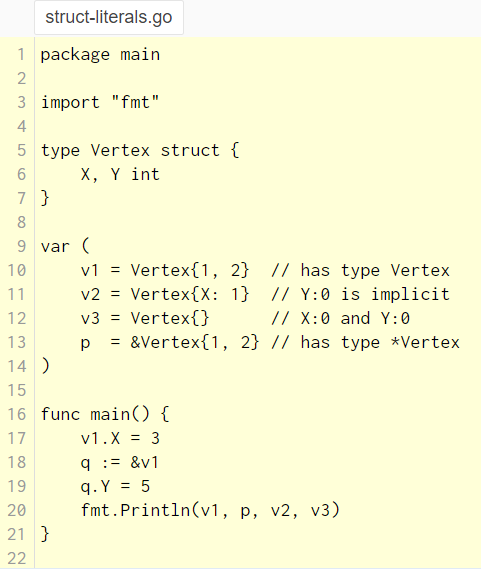
\includegraphics[width=0.9\linewidth]{img/struct.PNG}
        \end{column}
        \begin{column}{0.4\textwidth}
            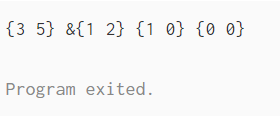
\includegraphics[width=\linewidth]{img/structoutput.PNG}
        \end{column}
    \end{columns}
\end{frame}
}

{
\begin{frame}
    \frametitle{Arrays}
    \begin{itemize}
        \item The type [n]T is an array of n values of type T
        \item An array's length is part of its type, so arrays cannot be resized
    \end{itemize}
    \begin{columns}
        \begin{column}{0.5\textwidth}
            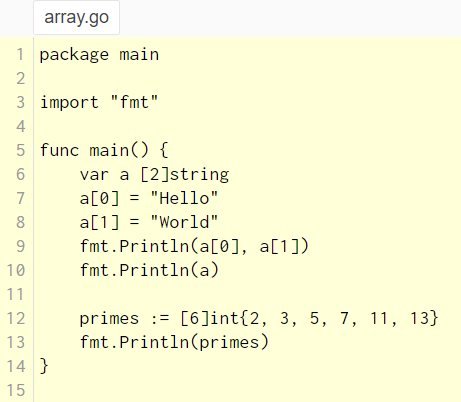
\includegraphics[width=\linewidth]{img/array.PNG}
        \end{column}
        \begin{column}{0.5\textwidth}
            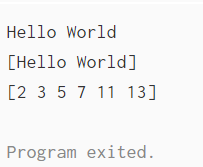
\includegraphics[width=0.5\linewidth]{img/arrayoutput.PNG}
        \end{column}
    \end{columns}
\end{frame}
}

{
\begin{frame}
    \frametitle{Slicing}
    \begin{itemize}
        \item Slicing of arrays is done the same way as in Python
        \item Slices are like references to arrays
    \end{itemize}
    \begin{columns}
        \begin{column}{0.5\textwidth}
            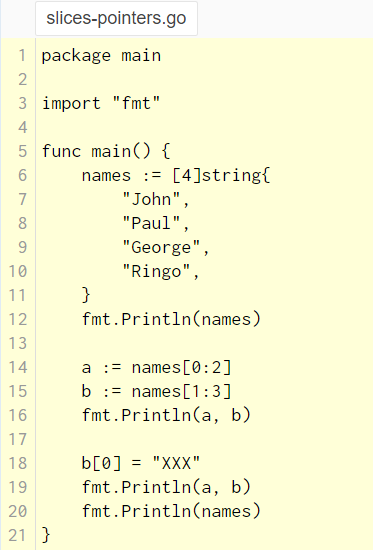
\includegraphics[width=0.7\linewidth]{img/slices.PNG}
        \end{column}
        \begin{column}{0.5\textwidth}
            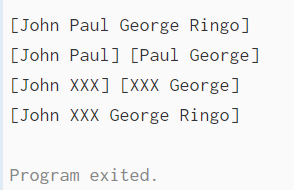
\includegraphics[width=0.7\linewidth]{img/slicesoutput.PNG}
        \end{column}
    \end{columns}
\end{frame}
}

{
\begin{frame}
    \frametitle{Slice Literals Length and Capacity}
    \begin{itemize}
        \item A slice literal is like an array literal without the length
        \item The length and capacity of a slice s can be obtained using the expressions len(s) and cap(s)
        \item There are also many more built-in functions like make and append that can be used with slices
    \end{itemize}
\end{frame}
}

{
\begin{frame}
    \frametitle{Slice Literals Length and Capacity}
    \begin{columns}
        \begin{column}{0.6\textwidth}
            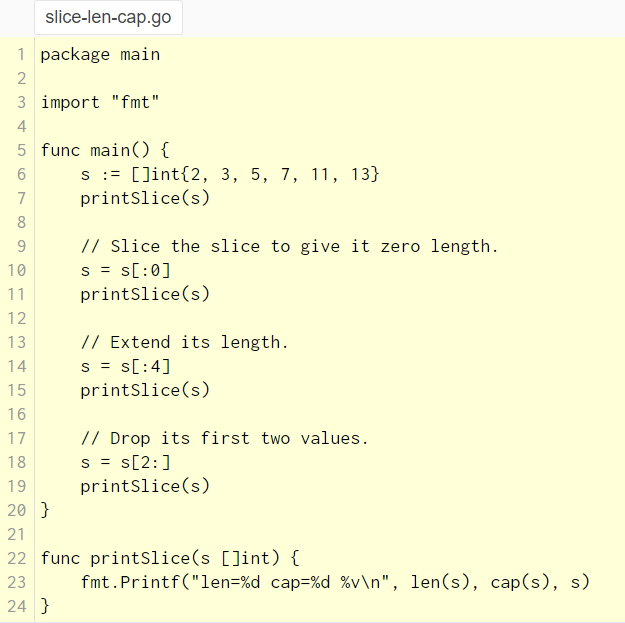
\includegraphics[width=\linewidth]{img/slicelencap.PNG}
        \end{column}
        \begin{column}{0.4\textwidth}
            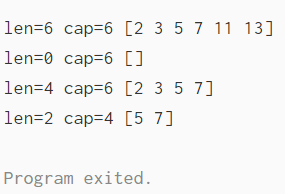
\includegraphics[width=\linewidth]{img/slicelencapoutput.PNG}
        \end{column}
    \end{columns}
\end{frame}
}

{
\begin{frame}
    \frametitle{Range}
    \begin{itemize}
        \item The range form of the for loop iterates over a slice or map
        \item two values are returned for each iteration, the index and the element at that index
        \item If you only want the index, you can omit the second variable
    \end{itemize}
\end{frame}
}

{
\begin{frame}
    \frametitle{Range}
    \begin{columns}
        \begin{column}{0.7\textwidth}
            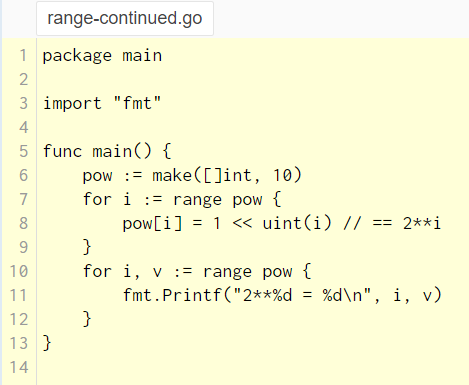
\includegraphics[width=\linewidth]{img/range.PNG}
        \end{column}
        \begin{column}{0.3\textwidth}
            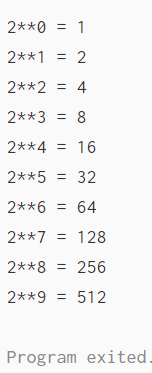
\includegraphics[width=0.7\linewidth]{img/rangeoutput.PNG}
        \end{column}
    \end{columns}
\end{frame}
}

{
\begin{frame}
    \frametitle{Maps}
    \begin{itemize}
        \item A map maps keys to values
        \item The zero value of a map is nil. A nil map has no keys, nor can keys be added
        \item The make function returns a map of the given type, initialized and ready for use
        \item We can also initialize maps using map literals
    \end{itemize}
\end{frame}
}

{
\begin{frame}
    \frametitle{Maps}
    \begin{columns}
        \begin{column}{0.55\textwidth}
            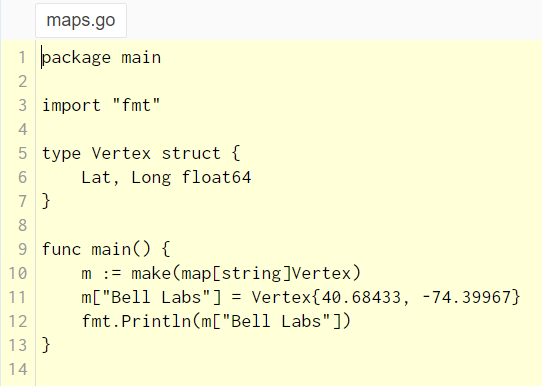
\includegraphics[width=\linewidth]{img/maps.PNG}
        \end{column}
        \begin{column}{0.45\textwidth}
            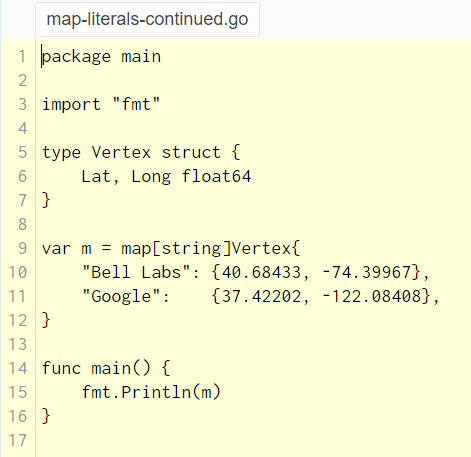
\includegraphics[width=\linewidth]{img/mapliterals.PNG}
        \end{column}
    \end{columns}
\end{frame}
}

{
\begin{frame}
    \frametitle{Maps}
    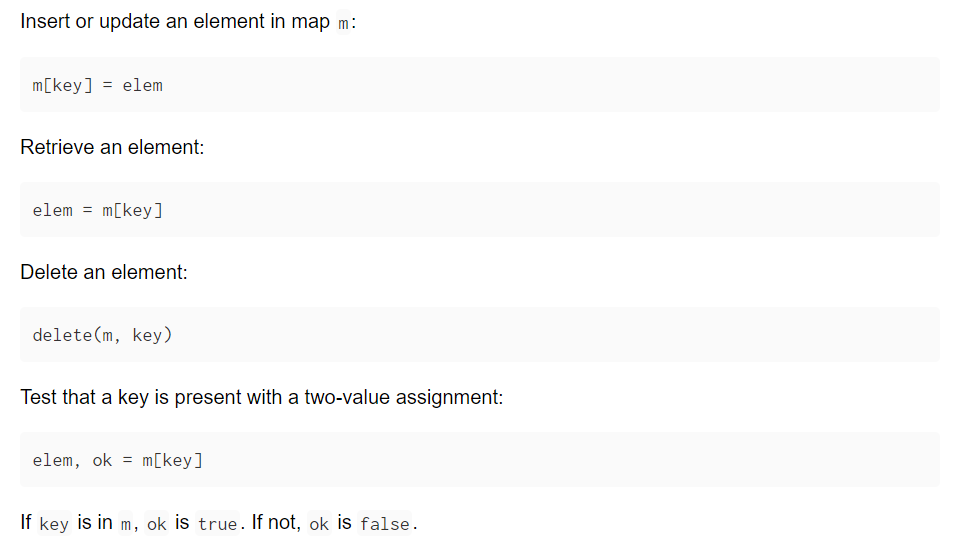
\includegraphics[width=\linewidth]{img/mutatingmaps.PNG}
\end{frame}
}

{
\begin{frame}
    \frametitle{Function Values}
    \begin{itemize}
        \item Function values may be used as function arguments and return values
    \end{itemize}
    \begin{columns}
        \begin{column}{0.6\textwidth}
            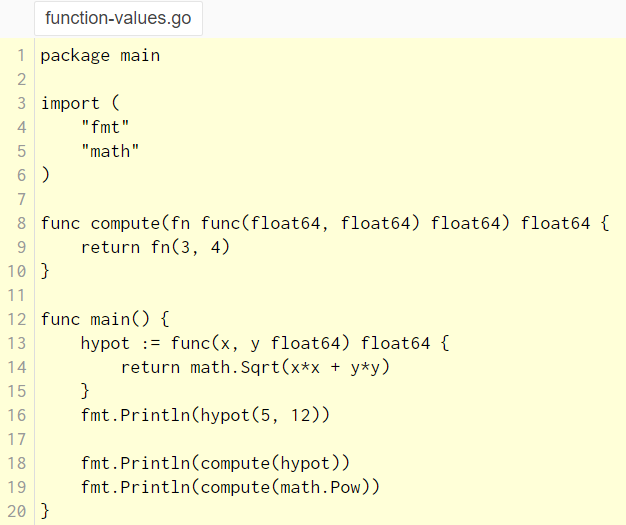
\includegraphics[width=\linewidth]{img/functionvalues.PNG}
        \end{column}
        \begin{column}{0.4\textwidth}
            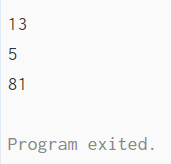
\includegraphics[width=0.6\linewidth]{img/functionvaluesoutput.PNG}
        \end{column}
    \end{columns}
\end{frame}
}

{
\begin{frame}
    \frametitle{Function Closures}
    \begin{itemize}
        \item A closure is a function value that references variables from outside its body
    \end{itemize}
    \begin{columns}
        \begin{column}{0.6\textwidth}
            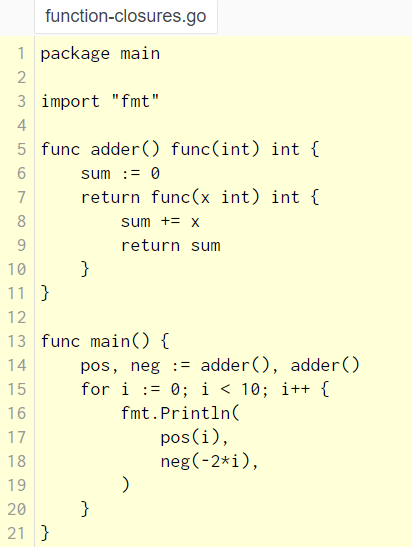
\includegraphics[width=0.65\linewidth]{img/functionclosures.PNG}
        \end{column}
        \begin{column}{0.4\textwidth}
            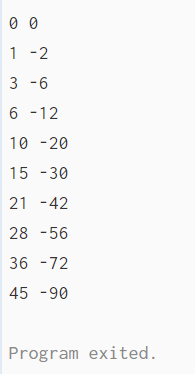
\includegraphics[width=0.5\linewidth]{img/functionclosuresoutput.PNG}
        \end{column}
    \end{columns}
\end{frame}
}

{
\begin{frame}
        
\includegraphics[width=\textwidth]{img/questions.PNG}
\end{frame}
}

\end{document}
